
\documentclass[article]{IEEEtran}
\usepackage[a5paper, margin=10mm, onecolumn]{geometry}

\usepackage{tfrupee} 
\setlength{\headheight}{1cm} 
\setlength{\headsep}{0mm}       
\usepackage{multicol}
\usepackage{gvv-book}
\usepackage{gvv}
\usepackage{cite}
\usepackage{amsmath,amssymb,amsfonts,amsthm}
\usepackage{algorithmic}
\usepackage{graphicx}
\usepackage{textcomp}
\usepackage{xcolor}
\usepackage{txfonts}
\usepackage{listings}
\usepackage{enumitem}
\usepackage{mathtools}
\usepackage{gensymb}
\usepackage{comment}
\usepackage[breaklinks=true]{hyperref}
\usepackage{tkz-euclide} 
\usepackage{listings}

\def\inputGnumericTable{}                                 
\usepackage[latin1]{inputenc}                                
\usepackage{color}                                            
\usepackage{array}                                            
\usepackage{longtable}                                       
\usepackage{calc}                                             
\usepackage{multirow}                                         
\usepackage{hhline}                                           
\usepackage{ifthen}                                           
\usepackage{lscape}
\begin{document}
	\title{10.6.8}
	\author{EE25BTECH11052 - Shriyansh Kalpesh Chawda}
	\maketitle
\textbf{Question}\\
(3,0) is the point from which three normals are drawn to the parabola \( y^2 = 4x \) which meet the parabola in the points \textbf{P}, \textbf{Q}, and \textbf{R}. Match the following \hfill (2006)

\begin{center}
	\begin{tabular}{c l c l}
		\hline
		& \textbf{Column I}  & &\textbf{Column II}  \\

		a) & Area of \( \triangle POR \) & a) & 2 \\
		b) & Radius of circumcircle of \( \triangle PQR \) & b) & \( \frac{5}{2} \) \\
		c) & Centroid of \( \triangle POR \) & c) & \( \left( \frac{5}{2}, 0 \right) \) \\
		d) & Circumcentre of \( \triangle PQR \) & d) & \( \left( \frac{2}{3}, 0 \right) \) \\
		\hline
	\end{tabular}
\end{center}

\textbf{Solution}\\
In matrix form,the parabola can be written as:
\begin{equation}
	\mathbf{x}^\top\myvec{0 & 0\\0 & 1}\mathbf{x} + 2\myvec{-2 & 0}\mathbf{x} + 0 = 0
\end{equation}
\begin{equation}
	V = \myvec{0 & 0\\0 & 1}, \quad u = \myvec{-2\\0}, \quad f = 0
\end{equation}

For point $h$ to lie on a normal to the conic, we use formula (10.1.9.1).

Let direction vector $m = \myvec{1\\m_1}$ and normal vector $n = \myvec{-m_1\\1}$.

\subsubsection*{Computing required terms:}

\begin{equation}
	Vh + u = \myvec{0 & 0\\0 & 1}\myvec{3\\0} + \myvec{-2\\0} = \myvec{0\\0} + \myvec{-2\\0} = \myvec{-2\\0}
\end{equation}

\begin{equation}
	\begin{aligned}
		g(h) &= h^\top Vh + 2u^\top h + f \\
		&= \myvec{3 & 0}\myvec{0 & 0\\0 & 1}\myvec{3\\0} + 2\myvec{-2 & 0}\myvec{3\\0} + 0\\
		&= 0 - 12 + 0 = -12
	\end{aligned}
\end{equation}

\begin{equation}
	m^\top(Vh + u) = \myvec{1 & m_1}\myvec{-2\\0} = -2
\end{equation}

\begin{equation}
	n^\top Vn = \myvec{-m_1 & 1}\myvec{0 & 0\\0 & 1}\myvec{-m_1\\1} = \myvec{-m_1 & 1}\myvec{0\\1} = 1
\end{equation}

\begin{equation}
	m^\top Vn = \myvec{1 & m_1}\myvec{0 & 0\\0 & 1}\myvec{-m_1\\1} = \myvec{1 & m_1}\myvec{0\\1} = m_1
\end{equation}

\begin{equation}
	n^\top(Vh + u) = \myvec{-m_1 & 1}\myvec{-2\\0} = 2m_1
\end{equation}

\subsubsection*{Substituting into (10.1.9.1):}

The condition for $h$ to lie on a normal is:
\begin{equation}
	\left[m^\top(Vh + u)\right]^2\left[n^\top Vn\right] - 2\left[m^\top Vn\right]\left[m^\top(Vh + u)\right]\left[n^\top(Vh + u)\right] + g(h)\left[m^\top Vn\right]^2 = 0
\end{equation}

Substituting values:
\begin{equation}
	(-2)^2(1) - 2(m_1)(-2)(2m_1) + (-12)(m_1)^2 = 0
\end{equation}

\begin{equation}
	4 + 8m_1^2 - 12m_1^2 = 0
\end{equation}

\begin{equation}
	4 - 4m_1^2 = 0 \implies m_1^2 = 1 \implies m_1 = \pm 1
\end{equation}
Additionally, $m_1 = 0$ (horizontal normal) is also a solution.
Therefore, the three slopes of normals are: $m = 0, 1, -1$\\
For parabola $y^2 = 4x$ (where $4a = 4 \implies a = 1$), if normal has slope $m$, the point of contact is:
\begin{equation}
	\left(am^2, -2am\right) = \left(m^2, -2m\right)
\end{equation}

\textbf{For $m = 0$:} 
\begin{equation}
	R = \myvec{0\\0}
\end{equation}

\textbf{For $m = 1$:} 
\begin{equation}
	P = \myvec{1\\-2}
\end{equation}

\textbf{For $m = -1$:} 
\begin{equation}
	Q = \myvec{1\\2}
\end{equation}
\subsubsection*{(a) Area of $\triangle PQR$}
Using the determinant formula:
\begin{equation}
	\text{Area} = \frac{1}{2}\left|\det\myvec{x_P & y_P & 1\\x_Q & y_Q & 1\\x_R & y_R & 1}\right|
\end{equation}

\begin{equation}
	= \frac{1}{2}\left|\myvec{1 & -2 & 1\\1 & 2 & 1\\0 & 0 & 1}\right|
\end{equation}

\begin{equation}
	= \frac{1}{2}\left|1 \cdot\myvec{1 & -2\\1 & 2}\right| = \frac{1}{2}|4| = 2
\end{equation}
Answer: Column II-a\\
\subsubsection*{(b) radius of circumcircle of $\delta$PQR}
Using the formula:
\begin{equation}
	R = \frac{|PQ| \cdot |QR| \cdot |RP|}{4 \cdot \text{Area}}
\end{equation}

\begin{equation}
	|PQ| = \left\|\myvec{1\\-2} - \myvec{1\\2}\right\| = \left\|\myvec{0\\-4}\right\| = 4
\end{equation}

\begin{equation}
	|QR| = \left\|\myvec{1\\2} - \myvec{0\\0}\right\| = \left\|\myvec{1\\2}\right\| = \sqrt{5}
\end{equation}

\begin{equation}
	|RP| = \left\|\myvec{0\\0} - \myvec{1\\-2}\right\| = \left\|\myvec{-1\\2}\right\| =\sqrt{5}
\end{equation}

\begin{equation}
	R = \frac{4 \cdot \sqrt{5} \cdot \sqrt{5}}{4 \cdot 2} = \frac{5}{2}
\end{equation}

Answer:Column II-b

\subsubsection*{(c) Centroid of $\triangle PQR$}

The centroid is given by:
\begin{equation}
	G = \frac{1}{3}\myvec{x_P + x_Q + x_R\\y_P + y_Q + y_R}
\end{equation}

\begin{equation}
	G = \frac{1}{3}\myvec{1 + 1 + 0\\-2 + 2 + 0} = \frac{1}{3}\myvec{2\\0} = \myvec{\frac{2}{3}\\0}
\end{equation}
Ans :Column II-d

\subsubsection*{(d) Circumcentre of $\triangle PQR$}
Since the triangle is isosceles with $|QR| = |RP| = \sqrt{5}$ and the points $P$ and $Q$ have the same $x$-coordinate with opposite $y$-coordinates, the circumcentre lies on the $x$-axis by symmetry.

Let the circumcentre be $O = \myvec{x_c\\0}$.

For circumcentre, the distance to all three vertices must be equal. Using vertices $P$ and $R$:
\begin{equation}
	|OP|^2 = |OR|^2
\end{equation}

\begin{equation}
	(x_c - 1)^2 + (-2 - 0)^2 = (x_c - 0)^2 + (0 - 0)^2
\end{equation}

\begin{equation}
	x_c^2 - 2x_c + 1 + 4 = x_c^2
\end{equation}

\begin{equation}
	-2x_c + 5 = 0 \implies x_c = \frac{5}{2}
\end{equation}
Answer: Column II-c

\subsection*{Final Matching}

\begin{center}
	\begin{tabular}{|c|c|}
		\hline
		\textbf{Column I} & \textbf{Column II} \\
		\hline
		a) & a) \\
		b) & b) \\
		c) & d) \\
		d) & c) \\
		\hline
	\end{tabular}
\end{center}

\begin{figure}[H]
	\centering
	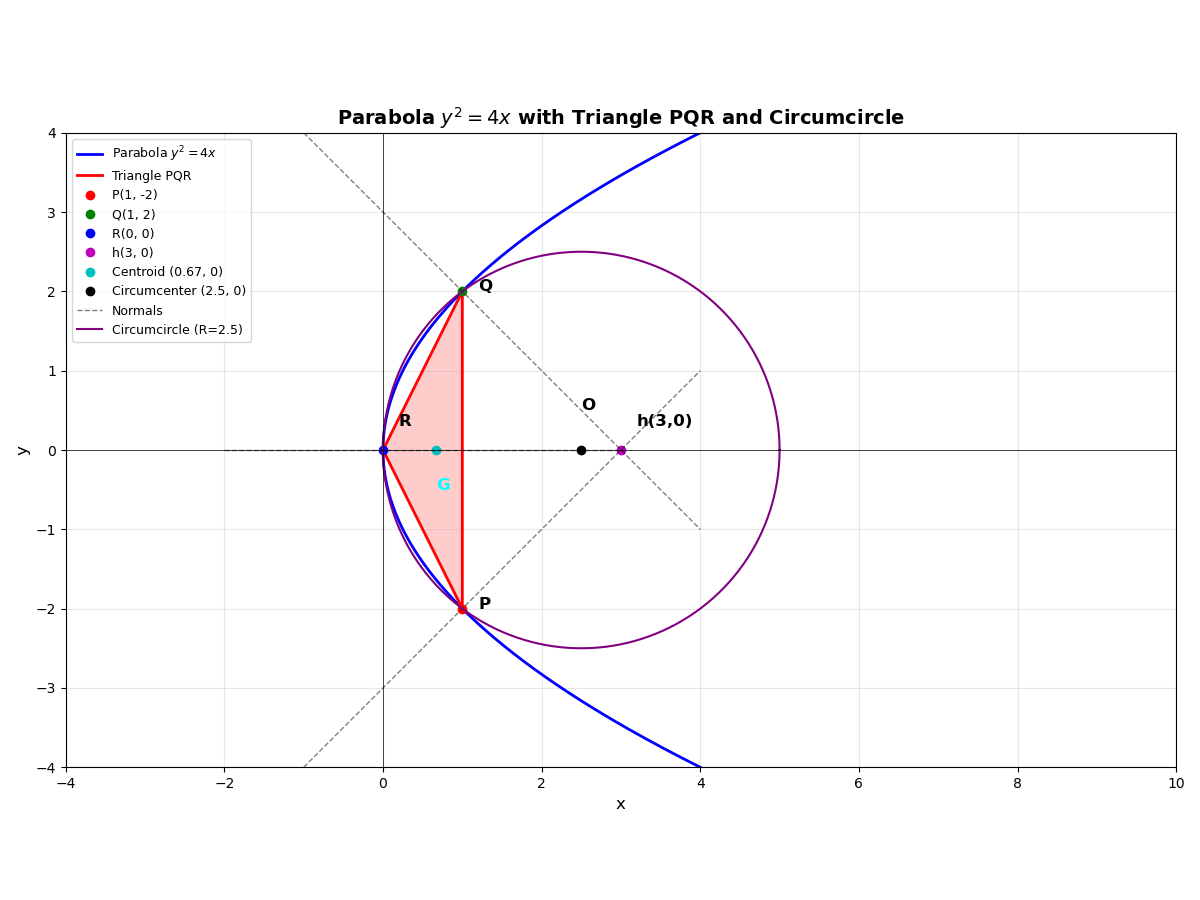
\includegraphics[width=1\linewidth]{figs/Figure_1}
	\caption{}
	\label{fig:figure1}
\end{figure}



\end{document}